\section{Database}
In this section we will present the design of our database.
Our design will support the concepts that we have introduced, namely project groups and project group members discussed in \secref{sec:projectgroup}.

Recall that we are designing to comply with a relational database, more specifically an SQL database as described in \secref{sub:constraints}.

\subsection{Project Group}
\label{sub:dbProjectGroup}
A project group is an entity that consists of different elements.
How these elements are represented in the database is presented here.
One core element is the project group members, this is described in \secref{sub:dbProjectGroupMembers}.
The other elements will be represented as fields in the \rel{projectgroup} relation.
%The reason for this is that a project group is an entity that has some attributes which we want to save persistent.

A project group must be identifiable by both human and computers.
To make a project group identifiable by humans we give it a short name that must be unique among other project groups.
The field that holds the short name in the project group relation is called \field{shortname}.
Initially it may seem that the short name could be used as a general identifier (both for humans and computers) since a short name is unique.
However, this name might be changed during the lifespan of a project group.
We would much rather prefer an identifier that is constant for a project group, to a avoid race conditions. 
%and violations of referential integrity
An example of a race condition in this system could be a user trying to access a project group with an identifier (the short name in this case) while another user is changing the short name of the group.
Should the short name be changed before the first user is trying to access the project group, the request will fail because the identifier that he is holding is deprecated.

We choose to have a numeric auto-incrementing \field{id} field to identify the project groups.
This cannot be set or changed by the users of the system.
%Ultimately a databse administrator could change it directly in the database, but we cannot guard gainst this assuming the database administrator has super user privelges.
It is a Moodle guideline to have an auto-incrementing field as primary key~\cite{moodledb}.
We clearly obey this guideline by making \field{id} the primary key of \rel{preojectgroup}.

One could argue that the numeric id field could be used as human identifier as well.
However, it is much easier for a humans to remember and associate an alphanumeric name with a particular project group than an arbitrary number.
In summary a project group has two identifiers; the numeric \field{id} and the alphanumeric \field{shortname}.
The former being the primary key of the relation.

To give a better description of a project group, we have an optional field called \field{longname}.
This field does not need to be unique, but only serve as a description for a project group.

To allow project groups to be ordered or filtered based on which semester, or similar, they belong to we choose to have a timestamp field called \field{created}.
The value of this field is the Unix-timestamp at the time of the creation of the project group.

The four fields of \rel{projectgroup} are as follows.
\begin{itemize}
	\item \field{id} to identify the group.
	\item \field{shortname} to easily identify the group for humans.
	\item \field{longname} of the group.
	\item \field{created} timestamp for a given project group.
\end{itemize}

\subsection{Project Group Members}
\label{sub:dbProjectGroupMembers}
As opposed to a project group a project group member is not an entity in its own right.
A project group member is a user that is a member of a project group.
\moodle{} saves users in a relation named \rel{user}.
This relation contains information about the users of the system -- a unique identifier in particular -- and is part of the \moodle{} core database schema~\cite{moodledbschema}.
We want project group members to be represented in the database as a link between \rel{projectgroup} and \rel{user}.
We want this link to be many-to-many, since a project group can contain many members and a user can be a member of many project groups.

We can save the link in either \rel{user} or \rel{projectgroup}, or create a new relation to save them in.
We state in our system definition (seen in \secref{sec:systemDef}) that current functionality of \moodle{} should not be altered.
The first alternative is therefore out of the question since we cannot guarantee that the other parts of \moodle{} will continue to work as before if we alter in the core database relations.

Should we choose the second alternative we would make $n$ fields in \rel{projectgroup}, each containing a member of the project group or a value indicating no members, e.g. as null.
This would set a maximum of $n$ members on every project group.
If there is a maximum number of members that will ever be in a project group and this number is acceptably low this alternative might be viable.
%We do not, however, know any such number.
The number of users in the system could be a candidate for a maximum value.
This number may, however, change as more users are added to the system.
Furthermore, this number is likely to be larger than the actual maximum number of members in any group, assuming that no or few projects are conducted by every user of a \moodle{} system.
Another option might be to choose a value that we believe is high enough for most purposes.
This would result in a many-to-$n$ link between project groups and users, in that a project group can have $n$ members and a user can be a member of any number of project groups.
If this $n$ value is chosen to high, space will be wasted, e.g. if $n$ is set to $20$ and no project group ever has more than 10 members, at least 10 fields in each \rel{projectrgoup} tuple will be wasted.
If $n$ is too low the system will be unacceptable because some desired project groups cannot be created.

The final alternative requires a new relation which stores a combination of users and project groups.
This allows for a true many-to-many link between users and project groups.
By choosing this alternative we have great extensibility, e.g. we are able to save the role of project group member in this relation as well.
A weakness to choosing this alternative is greater complexity by an increase in the number of relations.
The strengths of this alternative outweighs its weaknesses and it is better than the previous alternative by allowing a true many-to-many link without wasting space or making the system unacceptable.
Hence we choose this alternative as the way to save project group members in the database.
The relation that is used to link \rel{user} and \rel{projectgroup} is called \rel{projectgroup\_members}.

%%%%%%%%%%%%%%%%%%%%%%%%%%%%%%
% M�ske skal vi inds�tte en  %
% sub-subsection her         %
%%%%%%%%%%%%%%%%%%%%%%%%%%%%%%

For \rel{projectgroup\_members} to link \rel{user} and \rel{projectgroup} it will have a foreign key to both of these relations' primary keys.
The fields that hold these foreign keys are called \field{user} and \field{projectgroup} respectively.
The combination of \field{user} and \field{projectgroup} is a candidate key for \rel{projectgroup\_members}.
However, as with \rel{projectgroup} we choose to have a numeric auto-incrementing single field called \field{id} to comply with \moodle{} guidelines~\cite{moodledb}.
We still make the combination of \field{user} and \field{projectgroup} unique, to ensure that no person is a member of the same group twice or more.

Whenever a user is a member of a project group we want to have a role associated to that member.
We can choose to give every user a role and whenever that user is a member of a project group he can act and have privileges as fit for the role.
Another way to do it is to save the role along with the link between users and project groups.
We prefer the latter for two reasons.
Firstly a user may have different roles in different project groups, e.g. a Ph.D. student has a student role in his Ph.D. project, but may also be supervising projects being conducted by younger students.
Secondly we would have to make a new relation to contain only this information and thus increase complexity if the former alternative is to be chosen.
We will not alter the core relations such as \rel{user}, as described in \secref{sub:dbProjectGroup}.

To allow for extensibility we save the creation and update time of each tuple in \rel{projectgroup\_members} in \field{created} and \field{updated} respectively.
It may be useful to have these times for administrative personnel, e.g. to see whether or not a user has joined a project group later than the other members. \todo{Jeg har ingen anelse om hvorfor vi har disse med}

The final set of fields in \rel{projectgroup\_members} are:
\begin{itemize}
	\item \field{id} which is Moodle convention. \cite{moodledb}.
	\item \field{projectgroup} references to the related project group.
	\item \field{user} references to the related user.
	\item \field{role} denoting the type of membership the user has to the group.
	\item \field{created} is the timestamp for its creation.
	\item \field{updated} is the timestamp for the last update to the membership. 
\end{itemize}

The database scheme can be seen in~\figref{fig:projectgroupsdb}. 
The user entity is a build-in part of Moodle and is not modeled by us. 
\begin{figure}
	\centering
		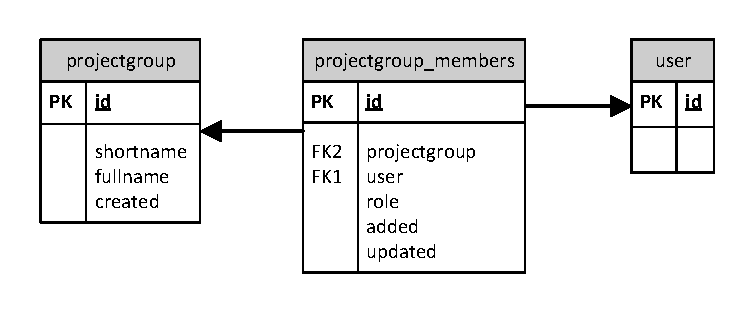
\includegraphics{images/projectgroupsdb.pdf}
	\morscaption{The database scheme of project groups and memberships. The data fields of the user table is omitted for brevity}
	\label{fig:projectgroupsdb}
\end{figure}

%To test the scheme for redundancy we check to see that the scheme conforms to boyce-codd normal form (BCNF). To check this we 

